\documentclass[mastersthesis,12pt]{wuthesis}     %% LaTeX2e document.
%
% Use one of the following
% \documentclass[mastersthesis,12pt]{wuthesis}
% \documentclass[dscthesis,12pt]{wuthesis}
% \documentclass[phdthesis,12pt]{wuthesis}
%
% If you want to use other packages such as amstex, or epsfig
% \usepackage them here.
%
% epsfig and ellipsis are 'packages' for LaTeX2e and
% should be part of your distribution.  If not talk to your
% sysadmin
\usepackage{epsfig}
\usepackage{ellipsis}
\usepackage{graphicx}
\usepackage{amsmath}
\usepackage{amssymb}
\usepackage{algpseudocode}
\usepackage[chapter]{algorithm}
\usepackage{xcolor}
\usepackage{siunitx}
\usepackage{wrapfig}

%%%%%%%%%%%%%%%%%%%%%%%%%%%%%%%%%%%%%%%%%%%%%%%%%%%%%%%%%%%%%%%%%%%%%%%%%%%%%
%%
%% These commands customize the `wuthesis' package for me
%%
%%%%%%%%%%%%%%%%%%%%%%%%%%%%%%%%%%%%%%%%%%%%%%%%%%%%%%%%%%%%%%%%%%%%%%%%%%%%%

%% Enter your official name
\renewcommand{\thesisauthor}{Emily Ramey}
\renewcommand{\thesisauthorlastname}{Ramey}

%% Enter your previous degrees
%% If you have no previous degrees remember to remove the comma too.
%\renewcommand{\thesisauthorpreviousdegrees}{, J.D.}

%% Enter department name
\renewcommand{\thesisdepartment}{Department of Computer Science and Engineering}
\renewcommand{\thesisfield}{Computer Science}

%% Enter date of graduation
\renewcommand{\thesismonth}{August}
\renewcommand{\thesisyear}{2019}

%% Enter title of thesis
\renewcommand{\thesistitle}{Event Reconstruction in the Advanced Particle-Astrophysics Telescope}
\renewcommand{\thesisshorttitle}{Event Reconstruction in the APT}

%% Enter the copyright holder ( DEFAULT is \thesisauthor )
\renewcommand{\thesiscopyrightholder}{\thesisauthor}

%% Enter supervisor name
\renewcommand{\thesissupervisor}{Dr. Jeremy Buhler}
\renewcommand{\thesiscommittee}{Jeremy Buhler \\
	James Buckley \\
	Roger Chamberlain}

%% Enter the dedication
\renewcommand{\thesisdedication}{Dedicated to my family, without whom none of this would have been possible. Thank you.}

%%%%%%%%%%%%%%%%%%%%%%%%%%%%%%%%%%%%%%%%%%%%%%%%%%%%%%%%%%%%%%%%%%%%%%%%%%%%%
%%
%% This paper is construced from other files.  Each \include'd file
%% begins a chapter.  This is done for easy developement and revision.
%%
%%%%%%%%%%%%%%%%%%%%%%%%%%%%%%%%%%%%%%%%%%%%%%%%%%%%%%%%%%%%%%%%%%%%%%%%%%%%%

\begin{document}

\frontmatter
%%
%  This is all that frontmatter stuff
%
%  This way I can 'not' include it easily

% NOTE: do not put any text in the thesistitlepage, thesiscopyrightpage,
% or thesisdedicationpage sections.  If you want to use these pages, then you
% should remove the notes below (e.g., by uncommenting the \iffalse
% and \fi lines) and change the appropriate fields in thesis-main.tex.
% This will ensure that the copyright and dedication lines are positioned
% and formatted correctly.  Additionally, remove the
% thesisacknowledgmentpostscript and listoftablespostscript sections, since
% these are used to add explanatory notes which shouldn't be there in normal
% theses.

\begin{thesistitlepage}               %% Generate the title page.
%\iffalse
\end{thesistitlepage}
\begin{extranotespage}
\iffalse
\begin{singlespace}
{ \textbf{Important - How to use this document:}} \\
This sample document outlines guidelines for the proper formatting of theses
and dissertations for Master's and D.Sc.\ degree seeking students within the
School of Engineering at Washington University.  (Ph.D.\ students can also make
use of this document; see special note below.)  This document is formatted
using the same guidelines which it describes.  Consequently, by making an extra
copy of this document you can use it as a template into which you can insert
your own thesis or dissertation textual matter, replacing the original text
with your own while still retaining the general formatting contained within.
This document/template can be downloaded (as either a Microsoft WORD document
OR as a set of \LaTeX{} files) from the Engineering Student Services' website
and is located with other engineering graduate forms and guides.  Once
completed, hard copies of your document will be submitted for professional
binding, plus you will also need to submit your copy electronically, as per
procedures documented on the Engineering website's information for graduate
students.  Be certain to use your own full name wherever appropriate.  After
removing these comments, be sure to vertically center the information on the
title page to assure an equal amount of ``white space'' exists both above and
below your general block of title page information; however, be sure to leave
the vertical spacing between each area of text on the title page exactly as
shown above.  Your examination committee will likely contain only three members
if you are a Master's student, as shown in the sample above.  However, D.Sc.\
committees will typically have five members, and Ph.D.\ committees will have
six.  Make sure you use the month and year your degree is officially to be
\uline{earned} on the title page, abstract page, and on any vita page included.
\uline{If this is for your doctoral degree (i.e., either D.Sc.\ or Ph.D.)}, be
sure to change all occurrences of the word ``thesis'' to display as
``dissertation'', and change ``MASTER OF SCIENCE'' to ``DOCTOR OF SCIENCE'' or
DOCTOR OF PHILOSOPHY'', whichever applies.   \\ \uline{IMPORTANT:  If you are a
Ph.D.\ student}, you must also change the line above (near the mid-section of
the title page) to ``A dissertation presented to the Graduate School of Arts and
Sciences'' (but do NOT change the reference to the ``School of Engineering''
which is at the very top of the title page, as that must be left exactly as shown.

{ \textbf{Note for Ph.D.\ Students:}} \\
The formatting contained within this sample document can serve well in
emulating the basic formatting needed for the Ph.D.\ dissertation.  Be sure to
read ``Important reminders'' in paragraph above.\\ However, please remember
that all Ph.D.\ students are ultimately responsible for meeting the Graduate
School of Arts \& Sciences' formatting guidelines.  The GSAS dissertation
guidelines are published on the Graduate School website located with other
documentation for GSAS policies and guides.

\end{singlespace}
\fi
\end{extranotespage}

\begin{thesiscopyrightpage}                 %% Generate the copyright page.
%\iffalse
\end{thesiscopyrightpage}


\begin{extranotespage}                        %% Students should not need this environment, it was added to insert pages with additional formatting instructions that should be removed by the student
\iffalse
\begin{singlespace}
\small{
{\textbf{Important Notes Regarding Copyright Option:}} \\
Technically, a thesis or dissertation is protected to some degree by copyright
laws with or without a student having to register his or her claim to
copyright.  However, including a copyright page and applying for registration
of ones claim to copyright provide extra measures of legal protection from
potential copyright infringement.  There is a fee connected with explicitly
registering to copyright ones work; because of this, many students do not
choose to register to copyright their work.  Students should check with their
advisor(s) and/or seek legal advice to gather further information helpful to
making a decision with regards to registering their claim to copyright.  If you
are \uline{not} going to register to copyright your work, then you can choose
to remove this page from your document.  However, if you do choose to
explicitly copyright your work, then leave this page in, change the name to
your name, change the year to the appropriate year in which your degree will be
earned, and remove these notes of informational text.  If a student wishes to
officially ``register'' this claim to copyright, then Masters students will
need to pursue that effort on their own and can find appropriate options by
searching the web.  Doctoral students can complete an authorization to apply
for registration (i.e., of their claim to copyright the dissertation) by
indicating this interest in the appropriate area on the online form when
submitting the final electronic copy as per procedures documented on the
Engineering website's information for graduate students.

{\textbf{Important Notes Regarding Page Numbering and Margins:}} \\
If you decide to include the copyright page in your final document, do
\uline{not} count the page among your counted pages, and do \uline{not} display
any page number on the page.  \uline{Every sheet of paper in the manuscript
should be numbered except for two:  the title page and this optional copyright
page.}  Specifically, the front textual information (which comes before your
main thesis/dissertation body of text) is numbered with Roman numerals, and
your main body of text begins with Arabic numbers.  Since the title page is
counted but \uline{not} numbered, roman numeral \uline{``ii'' is always the
first number used and appears on the page AFTER the title page (AND AFTER the
copyright page, IF included)} --- as shown in this sample template document.
Page numerals should always display centered, just above the 1 bottom margin.
The left margin should be 1.5 inches, with a 1 inch margin at top, bottom, and
right.  The left margin is extra-wide in order to accommodate the binding
process.  When typing the manuscript, stay well within these margin guides.
Lastly, remember to update your table of contents such that the page numerals
referenced there will match the page numbers on the bottom of the pages to
which they make reference in your document.  This is necessary to do manually
because, unfortunately, the page numbering within this templates table of
contents is \uline{not} automatically linked to the pages of the body of text.
This is further documented, along with some work arounds, in the appendix to
this guide called Special Notes for MS WORD Users.  \LaTeX{} users may have to
invent other solutions with regards to synchronizing table of contents page
references with actual document page numbers.  This guide merely provides a
helpful starting point.  \\ \textbf{REMINDER:} When you remove these comments, be
sure to leave the copyright information centered both vertically and
horizontally on the page (if you decide to explicitly copyright your work).}
\end{singlespace}
\fi
\end{extranotespage}


\begin{singlespace}
\setcounter{page}{2}
\tableofcontents

\iffalse
\renewcommand{\listoftablespostscript}{

\textbf{Note:} Be consistent in aligning multi-lined table-names, figure-names,
and chapter/section-names throughout your document.  It is generally
recommended to make sure any additional lines (i.e., within a long title or a
long table name) wrap and align immediately under the 1st character of the
title or name with which they are associated in the line immediately above ---
as shown in the ``Table 2.1'' example above.   Whatever approach you take, be
consistent.}
\fi

\listoftables

\listoffigures
\end{singlespace}

\iffalse
\renewcommand{\thesisacknowledgmentpostscript}{
\textbf{Reminders of what needs to be updated:}
After removing these comments, use the above format to help input your
acknowledgments page.   A special dedication can be placed as the final
paragraph, as shown above; alternatively, you may include a special dedication
on the page that follows, as also shown in this sample template.}
\fi

\begin{thesisacknowledgments}
I would like to thank my advisors, Dr. Jeremy Buhler, Dr. James Buckley, and Dr. Roger Chamberlain, for their support of my research. This material is based upon work supported by the National Science Foundation Graduate Research Fellowship under Grant No. 2018268910.

A special thanks goes to the many graduate students and distinguished faculty within the computer science and physics departments at Washington University who have reviewed this thesis and helped support the related research.
\end{thesisacknowledgments}
\iffalse
\begin{thesisdedicationpage} %% Generate the dedication page.

\textbf{Note:} You may include a special dedication as shown here.  If you
include this page, be sure to keep it brief and center it on the page both
horizontally and vertically.  Alternatively, you may remove this page
altogether, and a special dedication can be placed as the final paragraph to
your acknowledgments page (as shown in this document on the preceding page).
\end{thesisdedicationpage}
\fi

\begin{thesisabstract}

The Advanced Particle-Astrophysics Telescope (APT) is a concept for a gamma-ray space telescope that would operate in the keV to MeV energy range. Due to the nature of the telescope and the physics involved in detection, reconstructing initial photon trajectories through software can be very computationally complex, which is a barrier to the real-time detection of astrophysical transient phenomena such as Gamma Ray Bursts (GRBs) and supernovae. In this paper, we discuss several changes made to the basic Compton reconstruction algorithm discussed in Boggs \& Jean (2000) in order to achieve greater reconstruction speeds, and we investigate the effects of certain algorithmic parameters on computational performance. For testing, we create a simple toy model of Compton scatters in our detector and generate data from a uniform source distribution. Though less representative of nature, this allows for easier development of our algorithm and sets up a test framework for parameters of interest in future iterations of the project.

\iffalse

*** ask about abstract word limit for print indices!!!


\textbf{Reminders of what needs to be updated:} 
After removing these comments, begin typing the body of your abstract here,
\uline{double-spaced}.  The point-size of the body of the abstract can be set to
12 point (which is the text size of this sample comment-paragraph) or it can be
reduced to 10 point if you prefer.  Regardless of which specific point size you
select, the abstract must remain double-spaced and it should \uline{not} be
bolded.  \uline{If this is for your doctoral degree, be sure to change all
occurrences of the word ``thesis'' to display as ``dissertation'', and change
``Master of Science'' to ``Doctor of Science'' or ``Doctor of Philosophy'',
whichever applies.}  In the abstract heading above, make sure you \uline{use
the year your degree is officially to be earned}.  Be sure to use your full
name and your research advisor's full name wherever appropriate, and be certain
to use the correct title of your degree whenever referencing it. The title of
your degree will not always be the same as the title of your department or
program, so please check with your departmental administrative assistant and
advisor(s) to be sure you are using the correct degree title.  Questions you
may have about preparing your theses or dissertations are always welcomed at
the Office of Engineering Student Services.

\textbf{Length of Abstract:}
There is technically no word limit on your abstract.  Your abstract allows you
to describe your research in a section that can be accessible to search
engines, and therefore a word limitation would constrain potential exposure of
your work. However, from the electronic submission of theses or dissertations,
print indices may be published that will include references to abstracts. These
print indices require word limits of 350 words for doctoral dissertations and
150 words for master's theses. Additionally, these indices typically allow only
text to be included in the abstract. In the editorial process for these print
publications, the service provider will simply truncate your abstract if it
exceeds these word limits and remove any non-text content. You may wish to
limit the length of your abstract if this concerns you. The abstract as you
submit it will NOT be altered in your published manuscript.

\textbf{Note for Ph.D.\ Students:}
The formatting contained within this sample document can serve well in
emulating the basic formatting needed for the Ph.D.\ dissertation.   However,
please remember that all Ph.D.\ students are ultimately responsible for meeting
the Graduate School of Arts \& Sciences' formatting guidelines.  The GSAS
thesis and dissertation guidelines are published on the Graduate School web
site located with other documentation for GSAS policies and guides.  Be sure to
read all of the above notes/reminders on what needs to be updated as shown in
this template document's title, copyright, and abstract pages.  Ph.D.\ students
will submit final dissertations and all materials to the Office of Graduate
School of Arts and Sciences, and any questions about their dissertations should
also be directed to that office.
\fi
\end{thesisabstract}



\iffalse
\chapter{Preface}

This guide contains the School of Engineering's rules for formatting theses and
dissertations.\footnote{Throughout this guide, the word thesis refers to both
theses and dissertations.}   Departments, advisors, and committees may impose
additional rules.  In the past, students were required to study a similar (but
much longer) set of rules and apply them to their theses.  The Association of
Graduate Engineering Students (i.e., AGES) has helped to prepare templates and
style files that simplify thesis preparation.  These files have been set up to
produce acceptably formatted theses and dissertations using several popular
word processing and text formatting programs.  There should be one available in
Microsoft WORD and another in \LaTeX{}.  Students can retrieve these files and
their accompanying instructions from the Engineering Student Services' main
website.  Check with Engineering Student Services (Lopata Hall, Room 303) if
you have any questions.  Students who create their own templates or style files
are invited to submit these files for future use by others.

This guide you are now reading can be downloaded (in either MS WORD formatted
version or a \LaTeX{} version) and can be utilized as a template for formatting
your own theses.  In short, the margin settings, pagination, table of contents
logic, etc. are already established in the downloadable versions.  You can
simply replace the text within the template with your own text, thereby saving
you much setup time.

\textbf{NOTE:} \uline{This preface page is optional.  A preface page is usually
used to explain further details surrounding the background and motivation for
the work.  You can remove it completely}, but then be sure the reference to
this page is also removed from the Table of Contents.  The majority of students
do not include a preface page.

%%
%% For List of Abbreviations, Glossary or Nomenclature also
%% use \chapter, but put some kind of list environment inside.



%%% Local Variables: 
%%% mode: latex
%%% TeX-master: "thesis-main"
%%% End: 
\fi

\mainmatter
\chapter{Introduction}
\label{cpt:format}

% small blurb summary

\section{The APT}

The Advanced Particle-astrophysics telescope is designed to be a successor to the Fermi Gamma-ray Space Telescope, which has surpassed its expected mission time of 10 years. The main science objectives of the APT include studying high-energy transient phenomena such as supernovae and gamma-ray bursts (GRBs), continuing the search for dark matter, and conducting broader surveys of the sky in gamma rays. The APT would improve upon Fermi's sensitivity while maintaining a similar budget, allowing for a more extensive search for dark matter and an increased ability to detect transients.

\subsection{Hardware design}

The APT is designed to be used in the mid-keV to low TeV energy range, which is a significant improvement on Fermi's detecting range. The final telescope will consist of 20 repeated layers of detecting material, spaced 15 cm apart, in a cube 3 meters tall and 2.5 meters on each side. The middle section of each layer - the calorimeter - records the energy of each photon or particle that interacts with it, and the WLS fibers on the top and bottom of each layer record the corresponding position of each interaction. From this series of detected interactions, we are able to reconstruct the initial direction of the photon source using software.

\begin{figure}
    \centering
    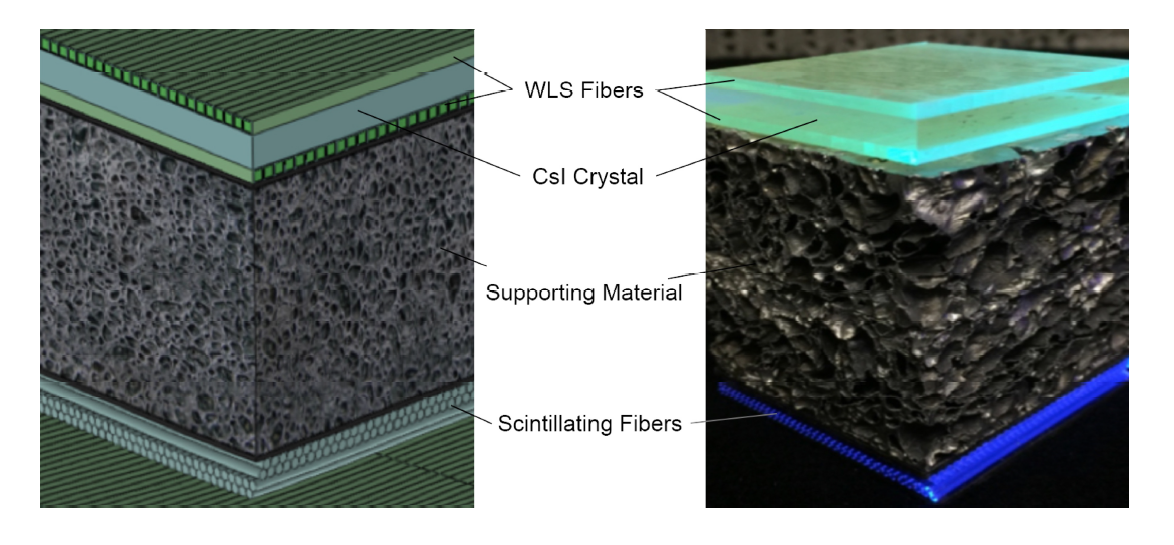
\includegraphics[width=0.7\textwidth]{APT_layers.png}
    \caption{One layer of the APT, shown as a computer model on the left and as a real-world prototype on the right, with aluminum used for the support structure. The Cesium Iodide (CsI) detects photon energy while the WLS fibers detect photon position. The scintillating fibers detect the position of any matter particles that enter the detector. Each subsequent layer would have the same structure as the one shown. \cite{APTmemo}}
    \label{fig:APT_layer}
\end{figure}

\subsection{Software design}
The APT achieves such a broad energy range by using two different software methods for reconstructing the trajectories of incoming photons, one for each of the two dominant gamma-ray interactions in this energy range. Below approximately 30 MeV, the dominant interaction is called Compton scattering, a process by which a photon transfers some portion of its momentum to an electron in a detector layer, changing its wavelength and trajectory. In the mid-MeV to GeV range, photons most commonly undergo a process called pair production upon interacting with the detector, in which a photon splits into a positron and an electron, which then interact further with the detector. As the goal of this project is to reconstruct Compton scatters, a thorough discussion of pair production is outside the scope of this paper, but a description of this phenomenon can be found in almost any particle physics textbook.

\section{Gamma-ray Bursts}
Though the APT can theoretically detect many types of transients, we focus primarily on gamma-ray bursts for this project. A gamma-ray burst (GRB) is an extremely bright burst of gamma-rays from a point source in the sky. These were first discovered in the 1960s by a US satellite that had been set up to detect radiation from nuclear blasts during the Cold War. The Compton Gamma-Ray Observatory (CGRO), launched in 1991, was used to determine that GRBs originate mainly from outside the Milky Way, and the Fermi Gamma-Ray Space Telescope, launched in 2008, has increased our understanding of the processes that cause these highly energetic blasts. A GRB can last anywhere from a few milliseconds to several hours, which is an incredibly short time window compared to most other astronomical observations. Many astrophysicists now believe that short-duration GRBs are caused by neutron-star mergers (collisions of extremely dense stellar remnants), while longer-duration GRBs originate from core-collapse supernovae (explosions of high mass stars), however much remains a mystery about how and why these events occur.

\section{This project}
\subsection{Motivation}
Though several theories exist as to their causes, the emission mechanisms of GRBs are not yet well-understood. The energies involved indicate a very efficient conversion of matter to energy, the process that drives this conversion is still an open question in the field of astrophysics. To better understand the processes that produce GRBs, it would be highly useful to observe them simultaneously with multiple different telescopes at multiple different wavelengths (gamma-ray, optical, infrared, etc.) To do this, we must be able to search for and detect a GRB in its initial stages and send out its location to other observatories. Achieving this goal could lead to future discovery in the field of astrophysics as GRBs become better understood.

One major science objective of the APT is to process gamma-ray events quickly enough to localize a source within a few seconds of the start of the burst and signal its location in that time. This means that we must significantly increase the detection capabilities of the APT in the low-energy range (keV - MeV) such that the incoming photons' directions can be reconstructed as quickly as they are received by the detector. As Compton scattering is the dominant interaction at these low energies, the primary focus of this research is to develop and test an algorithm to reconstruct Compton-scattered photons quickly and accurately enough that the telescope can pinpoint their source in close to real time. Many Compton telescopes rely on photon events with only two interactions to reconstruct their source positions. However, a significant fraction of events in this low energy range will scatter twice or more in the detector, which means that we can achieve significant performance improvement by incorporating the reconstruction of multi-scatter events into our algorithm.

\subsection{Scientific Constraints}

To eventually reach the main goal of this project, several factors be taken into account at this stage. The telescope must be able to reconstruct the trajectories of gamma rays at or near the speed at which they enter the detector, with low latency between the initial detection signal and the reconstructed solution. We expect to see between $10^5$ and $10^9$ photons per second during a typical gamma-ray burst\cite{UMD}. Our goal for reconstruction speed is $\backsim 10^5$ photons per second, with $>75\%$ accuracy and a latency of 1 second or less, as we expect this will give us an accurate enough localisation of the source position, but more complex simulations and source reconstructions will allow us to further constrain these target values. One of our other concerns is power consumption - the telescope will be part of a larger scientific instrument with a fixed amount of energy available to it daily. As such, we estimate that it cannot use more than 50 watts of power when running the reconstruction software.

\subsection{Process}
We base our initial Compton reconstruction algorithm on \emph{Boggs \& Jean (2000)}\cite{Boggs} and, with several performance improvements, we are able to meet our performance goals for this project. We start with a sequential algorithm, which enumerates each possible ordering of detector hits, and improve its performance by incorporating a tree search and pruning methods to improve the runtime. We build a simple gamma ray simulator for our development and initial tests of reconstruction speed and accuracy. Initial tests show that, with average parameters, the algorithm is able to reconstruct $\backsim 10^5$ photons per second with 80-90\% accuracy, which we believe will be enough to detect and localize a gamma-ray burst once the telescope is operational. By varying parameters in the algorithm, we also examine trends in the speed and accuracy, and discuss some possible trade-offs between the two, as well as possible improvements to the speed and accuracy for future work.

\section{Related Work}
One of the best papers available on Compton reconstruction procedures is \emph{Boggs \& Jean} (2000)\cite{Boggs} which details the mathematical formulae and steps required to reconstruct the initial direction of a Compton event in a layered detector. Though the paper focuses more on the physics of reconstructing Compton scatters than the algorithmic parameters, the equations listed served as a very helpful starting point for building and refining our code. We developed with the purpose of creating an algorithm to be as fast and lightweight as possible while still meeting our accuracy requirements. Many Compton telescopes must transfer data over a network connection or save observations in order to reconstruct them later, but our program is designed to process data in real time, before it leaves the telescope.

\iffalse
- Boggs \& Jean
        - focused more on the physics than the CS
        - Gives us a basic algorithm to improve upon
- Zoglauer's Megalib
- COMPTEL
    - It uses Compton scattering to detect GRBs, like our detector
    - But it only has two layers (lower probability of interaction) and as such it can only detect two-scatter events, a small fraction.
    - Has a good signal-to-noise ratio, which may be harder to emulate with the APT as it has a much larger detecting area
    - Might be more easy to determine polarization with more layers - Compton scattering is sensitive to photon polarization, so more Compton scatters would give us more chances to determine if the scattering angles have a preferential direction \cite{COMPTEL}.
    - It also has a Time Of Flight detector, which our telescope lacks
    - They also used Geant for testing
- COSI
    - It is also a multiple compton scattering detector
    - flies up on a balloon instead of being space-based
- MEGALib
    - basically the exact same thing as our algorithm but better
    - Realta package can reconstruct Compton events in real time
    - As far as I can tell, the only difference is you need an internet connection
\fi
%
%\addtocontents{toc}{\newpage}
\chapter{Compton Reconstruction}

\section{The physics of Compton scattering}

\begin{figure}
    \centering
    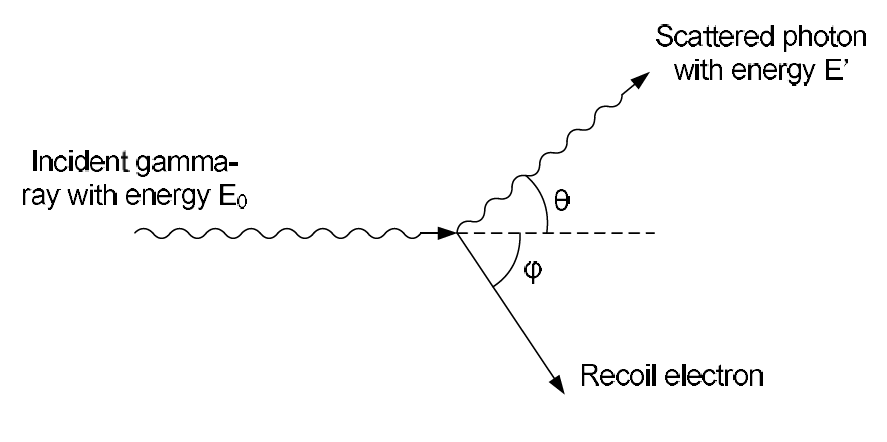
\includegraphics[width=0.7\textwidth]{Compton_scatter.png}
    \caption{Diagram of the Compton scattering process. \cite{comptonThesis}}
    \label{fig:compton_scatter}
\end{figure}

Compton scattering is a process in which a photon hits a charged particle and transfers some momentum to it in the collision. Due to conservation of momentum and energy, the photon moves away from the collision with a different wavelength and direction than it had initially, shown in Figure \ref{fig:compton_scatter}. In the APT, gamma rays from space scatter off of bound electrons in the detector material and kick them out of the layer that they had previously occupied. The gamma ray's energy can then be described with Equation \ref{eq:compton}:

\begin{equation}
    \label{eq:compton}E' = \frac{E_0}{1+\frac{E_0}{m_ec^2}(1-\cos\theta)}
\end{equation}

Where $E'$ is the energy after the collision, $E_0$ is the energy before the collision, $\theta$ is the scattering angle of the photon, and $m_e$ is the mass of the electron. Note that the scattering angle, the initial energy, and the final energy are the only free parameters in this equation, so determining any two of these values also determines the third. In reconstruction, we use the total energy deposited in the detector as the initial energy and are able to infer the energy and angle of each scatter from there.

Equation \ref{eq:compton} is based on the assumption that the electron is at rest in the detector material prior to the collision. The effects of the electron's initial momentum lead to a phenomenon called Doppler Broadening in the resulting Compton spectrum, which causes some error in our calculations. However, this effect is relatively small ($\backsim$0.01\% of initial wavelength) and randomly distributed, so we do not take it into account in our initial calculations, though it may be useful to do so in future work.

% \section{Photon Detection} can expand if low on text

\begin{figure}
    \centering
    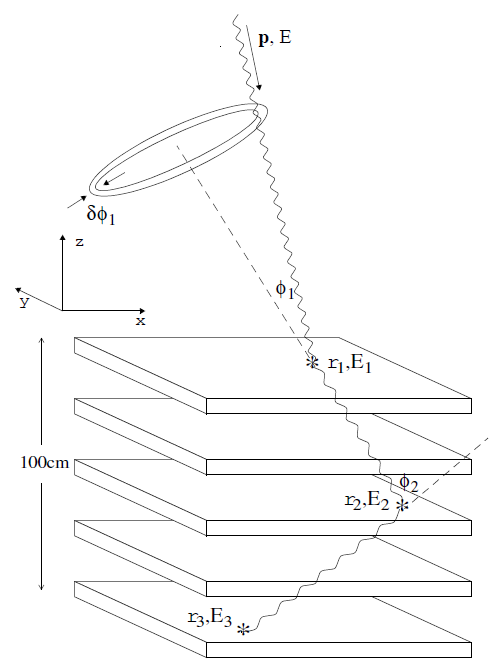
\includegraphics[width=0.3\textwidth]{detector_scattering.PNG}
    \caption{An example event showing a gamma-ray's trajectory through detector layers. Each * symbol is one hit. The dotted line shows the center of the cone of possibility while the wavy line represents the true path of the gamma-ray. \cite{comptonThesis}}
    \label{fig:scatters}
\end{figure}

\section{Reconstructing photon direction}

Photons are measured in the APT as a series of energy deposits, or \emph{hits}, in the detector material, as shown in Figure \ref{fig:scatters}. The final hit is assumed to be a photo-absorption, in which the photon is absorbed into the detector material instead of scattered off an electron. Each time the photon scatters, it deposits some energy in the detector, which is recorded through the scattered electron. It will then either scatter again or undergo photo-absorption, with the relative probability of each process depending on the remaining energy. From Equation \ref{eq:compton}, if we know the scattering energy and positions of the first two hits, we can use these to calculate the initial scattering angle of the photon. However, this does not give us the exact trajectory of the incident photon, but rather the "cone of possibility", defined by the scattering angle and the direction we record for the scattered photon. When taken for many photon events, these values can be used to extrapolate the position of the initial gamma-ray source.

If we already knew which hits came first in each sequence, or \textit{event}, we could get the initial scattering angle of the photons with a simple calculation. However, the biggest challenge in reconstructing photon trajectory is the fact that the detector cannot give us the chronological ordering of hits. Each gamma-ray moves at the speed of light, and the distance between detector layers is small enough that we would need a much higher time resolution to determine the first two hits chronologically. However, Equation \ref{eq:compton} allows us to infer the correct ordering in a different way, by comparing the spatial angles between the recorded hits to the scattering angles implied by their respective energy deposits. If there were no other factors involved, each correct spatial angle would have an exact match in energy angle, but detector noise and electronic effects mean that we must take a probabilistic approach to finding the correct sequence.

\section{Methodology}
To make things simpler in our code, we break each photon's series of hits into triples, one for each possible sequence of three hits. Each triple has a spatial angle - such as $\phi_2$ in Figure \ref{fig:scatters} - and an energy angle, which is calculated by Equation \ref{eq:compton} using the summed energy deposits of the sequence. One obstacle to our calculations is that the implied scattering angle does not depend on the energy deposited at the vertex of a given triple, but on the total energy of the photon both before and after the hit at the vertex. This means that we cannot calculate the energy angles individually, but only as part of a sequence. If we change the hits in the sequence before a given triple, it changes the energy calculations for the triple itself. To describe these constraints mathematically, we use equations adapted from Boggs \& Jean (2000)\cite{Boggs}:

\begin{align}
    W_i &= \frac{1}{m_ec^2}\sum_{j=i+1}^N E_j & \text{Unitless energy}\\
    \label{eq:new_compton}\eta'_i &= \cos\theta' = 1+\frac{1}{W_i}-\frac{1}{W_{i+1}} &\text{Energy angle}\\
    \eta_i &= \cos\theta = \hat{r}_i \cdot \hat{r}_{i+1} &\text{Spatial angle} \label{eq:eta}\\
    \hat{r}_i &= \frac{\vec{x}_i - \vec{x}_{i-1}}{|\vec{x}_i - \vec{x}_{i-1}|} & \text{Direction before hit $i$}
\end{align}

Where $N$ is the event's total number of hits in the detector and $W_i$ is the unitless energy of the photon after hit $i$ (i.e. $W_0$ is the initial energy of the photon and $W_{i>0} < W_0$). Equation \ref{eq:new_compton} is just a reformulation of the original Compton equation (\ref{eq:compton}) with $\theta'$ representing the energy scattering angle at hit $i$. $\theta$ is the spatial angle of hit $i$, and is calculated using a dot product, where $\vec{x}_i$ refers to the position of hit $i$ and $\vec{r}_i$ is the vector between hit $i-1$ and hit $i$. Therefore $\hat{r}_i$ is the direction of the photon immediately before hit $i$, and $\hat{r}_{i+1}$ is its direction immediately after. As finding the inverse cosines of Equations \ref{eq:new_compton} and \ref{eq:eta} can cost us valuable computation time, we leave them in their cosine form, $\eta$ and $\eta'$, and compare these values rather than the values of the angles themselves. The cosine function is uniquely determined for $\theta, \theta' \in [0 2\pi)$, so the two operations are mathematically equivalent.

\subsection*{The $\chi^2$ metric}
To compare the spatial and energy angles of a given sequence of hits, we use a $\chi^2$ test:

\begin{equation}
    \label{eq:chi2}\chi^2 = \frac{1}{N-2} \sum_{i=2}^{N-1} \frac{(\eta_i-\eta_i')^2}{\delta\eta_i^2+\delta\eta_i'^2}
\end{equation}

Where $\eta_i$ and $\eta_i'$ again represent the spatial and energy angles and $\delta\eta_i$ and $\delta\eta_i'$ represent the error in the spatial and energy angles. An example graph of this distribution can be found in Figure \ref{fig:p-val}.

The $\chi^2$ distribution is a sum of squared Gaussian distributions, so if we assume our noise/error, $(\eta_i-\eta_i')$, has an approximately Gaussian distribution, we can use the $\chi^2$ metric with $N-1$ degrees of freedom (the total number of hits) to determine the likelihood of a given ordering of hits. We can see by the equation that if the spatial and energy angles of any given triple match more closely, the value of $\chi^2$ will be lower, whereas if they are farther apart it will be higher. Therefore, in the absence of other factors, the sequence of hits that matches our data best will be the one with the lowest $\chi^2$ value. As the factors that affect our noise and error levels result from complicated physical processes, the true noise distribution may not be perfectly Gaussian. However, based on the Central Limit Theorem\cite{CLT} and a reasonable assumption of the number of independent variables that can affect our angle calculations, we can say that a Gaussian distribution is likely a reasonable approximation for our overall error.

\iffalse

This chapter describes the components of a thesis.  You need not include all
components described here, but you must follow the prescribed order for the
components you do include. Table~\ref{tab:components} lists the required and
optional components in the order that they should appear.  Your thesis should
include three main parts: the front matter, the text, and the back matter.
Each of these parts is described below.

\section{Front Matter}

The front matter includes all material that appears before the beginning of the
main text.  Number all ``front matter'' pages (except the title page and the
optional copyright page) with lower-case roman numerals, centered just above
the bottom margin.  Each of the following sections should begin on a new page.

\subsection{Title Page}

Format the title page so that it is centered vertically and horizontally on the
page with equal amounts of white space from top and bottom margins.  Include a
1.5-inch left margin and a 1-inch right margin.  Use a 12- or 14-point regular
Garamond, Times or Roman font on this page.  If you are writing a dissertation,
substitute the word ``dissertation'' wherever the word ``thesis'' appears in
this document.  The date on the title page should reflect the month and year
the degree will be awarded and should be one of the following months: December,
May, or August.  Do \uline{not} number the title page.

\begin{table}[ht]
\refstepcounter{table}
\label{tab:components}
\centering
Table \ref{tab:components}: Required and Optional Thesis Components
\addcontentsline{lot}{table}{\numberline{\ref{tab:components}}{%
	\ignorespaces Required and Optional Thesis Components
	(NOTE: If you have a multi-lined table label/title, then the 2nd and
	all additional lines should align with the first line, just like this
	one; plus, be sure that no words display to the far right hand side
	where the page numbers for your tables display, just as shown in this
	example.)}}

% Note: the \addcontentsline is a hack to force LaTeX to add a different
% entry to the text and table-of-contents.  Don't do this normally.

\vspace{0.125in}
\begin{spacing}{1}
\begin{tabular}{| c | c | c | c|}
\hline 
\textbf{Major Part} & \textbf{Thesis Component} & \textbf{Required}
 & \textbf{Optional} \\ \hline

\textbf{Front Matter} & Title Page & $\bullet$ & \\ \cline{2-4}
 & Abstract Page & $\bullet$ & \\ \cline{2-4}
 & Copyright Page & & $\bullet$ \\ \cline{2-4}
 & Dedication & & $\bullet$ \\ \cline{2-4}
 & Table of Contents & $\bullet$ & \\ \cline{2-4}
 & List of Tables & (Rqrd if used) & \\ \cline{2-4}
 & List of Figures & (Rqrd if used) & \\ \cline{2-4}
 & List of Abbreviations & & $\bullet$ \\ \cline{2-4}
 & Glossary of Nomenclature & & $\bullet$ \\ \cline{2-4}
 & Acknowledgments & & $\bullet$ \\ \cline{2-4}
 & Preface & & $\bullet$ \\ \hline

\textbf{Text} & Chapters & & $\bullet$ \\ \hline

\textbf{Back Matter} & Appendices & & $\bullet$ \\ \cline{2-4}
 & References & $\bullet$ & \\ \cline{2-4}
 & Vita & $\bullet$ & \\ \cline{2-4}
 & Short Title Page & $\bullet$ & \\ \hline
\end{tabular}
\end{spacing}
\end{table}

\subsection{Copyright Page}

Include a copyright page if you plan to copyright your thesis.  If used, the
copyright page must be unnumbered, immediately following the title page.  It
should include three lines, centered on the page with regular body text font
and spacing.  The 1$^{st}$ line should be ``copyright by'', the 2$^{nd}$ line
should contain your full name.  The 3$^{rd}$ line should contain the year the
degree is to be awarded.  Do not number the copyright page.  If you are a
Master's candidate and would like to register your claim to copyright your
thesis, you must make all arrangements independently.  Doctoral students will
complete a publishing agreement form which will give them a copyright
registration option.

\subsection{Abstract Page}

Please see important note regarding length of abstract found near the front of
this guide within the sample abstract.  Format the abstract page precisely as
done in this document.  The abstract page \uline{always} begins the document's
page numbering at ``ii''.

\subsection{Acknowledgments}

An acknowledgments section should be included..  Use it to thank those who
supported your research through contributions of time, money, or other
resources.  Type the word ``Acknowledgments'' in chapter title style at the top
of page.  If the acknowledgments fill more than one page, put the heading only
on the first page.  Number the page with a Roman numeral, centered at bottom,
sequentially following the abstract page(s) Roman numeral(s).

\subsection{Dedication}

The dedication page is optional.  If you decide to include a separate
dedication page,  make it short and center it on the page.  If included, you
should number it, placing the next logical/sequential Roman numeral at bottom
of page, centered, as shown in this sample document.

\subsection{Table of Contents}

The table of contents must include the page numbers of all chapters and
sections of your thesis.  In addition, it may include the page numbers of all
subsections.  It must also include the page numbers of all front and back
matter elements, unless otherwise specified.  Chapter titles should appear
flush left, section headings may be indented up to 0.5 inch, and subsection
headings may be indented up to 1 inch.  Chapter titles may be typed in plain or
bold font.  All titles and headings must be followed by a dot leader and a page
number.  The word ``Contents'' must appear in chapter title style at the top of
the page.  Be sure to align multi-lined chapter titles in the table of
contents.  For example, when a table of contents' chapter or section title
extends to a second line, be sure that the 1st character of the 2nd line aligns
immediately under the 1st character of the title/chapter/section name on the
line above it (i.e., as done in this sample document's table of contents, and
as specifically illustrated in the ``list of tables'' page for
table~\ref{tab:components}).  Make certain, too, that these long titles also
align nicely within the body of text, where multi-lined chapter titles or
section titles should still break at a logical point and align in a manner
allowing the titles to be read clearly without confusion.  Sometimes, for long
chapter or section titles, this will mean forcing a line break at a logical
point.  This cannot be automated, but relies on your own good judgment.  A good
example of a multi-lined title can be found at the top of
Appendix~\ref{app:english-language}; notice how the two lines are deliberately
divided helping each phrase to be read easily and fluidly.

\subsection{List of Tables}

Include a list of tables only if your thesis actually contains tables.
Format the list of tables the same way the table of contents is
formatted, but put the word ``List of Tables'' in the heading.

\subsection{List of Figures}

Include a list of figures only if your thesis actually contains
figures. Format the list of figures the same way the table of contents
is formatted, but put the word ``List of Figures'' in the heading.

\subsection{List of Abbreviations}

Include a list of abbreviations only if you use abbreviations that are
not common in your field.  Arrange the list alphabetically.  Type the
word ``List of Abbreviations'' in chapter title style at the top of the
page.

\subsection{Glossary or Nomenclature}

Include a glossary or nomenclature section only if your thesis
contains technical words that are not commonly used by people in your
field.  Type the word ``Glossary'' or ``Nomenclature'' in chapter title
style at the top of the page.  The glossary or nomenclature section
should consist of an alphabetized list of words and their definitions.

\subsection{Preface}

A preface is optional.  If you include a preface, use it to explain the
motivation behind your work.  Format the preface the same way the
acknowledgments section is formatted, but use the word ``Preface'' in the
heading.

\section{Text}

The text part of the thesis should be divided into numbered chapters, sections,
and subsections.  Use Arabic numerals for this numbering.   Divisions smaller
than subsections may be used, but they should not be labeled with numbers.
Place Arabic page numbers throughout the body of text centered just above the
bottom margin.

\section{Back Matter}

Throughout the back matter, use the same Arabic page number formatting as used
in the body of text section.

\subsection{Appendices}

Appendices may be used for including reference material that is too lengthy or
inappropriate for the thesis text.  If one appendix is included, an appendix
title is optional.  If more than one appendix is included, each one should be
titled and lettered.  In general, appendices should be formatted like chapters.
However, they may be single spaced or include photocopied material.  If
photocopied material is used, you must add page numbers at the bottom, putting
those page numbers in square brackets to indicate that they are not part of the
original document.

\subsection{References}

The reference section should follow the final appendix (or the conclusion of
the text if there are no appendices).  Type the word ``References'' in chapter
title format at the top of the page.  Single space within references and double
space between them.  More information on formatting references is included in
Chapter~\ref{cpt:citation}.

\subsection{Vita}

Including a vita page with your thesis is optional.  If you choose to include a vita
page, it should include your name, relevant academic and professional achievements,
and current month and year you will be earning your degree.  It may also include your
publications and professional society memberships.  If included, your vita should be the 
last page of your thesis.  Note: Personally identifiable information such as birth date
and place of birth should not be included on this page.

\subsection{Short Title Page}

The short title page should be prepared as described in
Appendix~\ref{app:procedures}.

\fi

%%% Local Variables: 
%%% mode: latex
%%% TeX-master: "thesis-main"
%%% End: 

\chapter{The Reconstruction Algorithm}

\section{Basis}

Our reconstruction uses the $\chi^2$ metric to determine which ordering of hits is best. Each triple represents one term in the sum of Equation \ref{eq:chi2}. Since we assume that the ordering with the lowest $\chi^2$ value is the correct one, we must try each possible ordering of hits in order to find it, which is very computationally complex. Our initial pseudocode for this calculation is shown in Algorithm \ref{alg:seq}. If there are $N$ hits in a photon event, there are $N!$ possible orderings of those hits, and we must recalculate the $\eta$ value for each hit in each ordering, adding an additional factor of $N$, to give us a total run-time of $O(N*N!)$ for each photon. There are several heuristic improvements we can make to shorten the average-case run-time, but we start with a basic iterative and sequential approach for simplicity's sake.

\subsection{Data types}
Data for each hit of each event is saved in a \texttt{Hit} data type, containing an x, y, z position and the energy deposit in MeV. Each photon which interacts with the detector is represented as an \texttt{Event} data type, which contains an array of \texttt{Hit} values and the number of hits total for that photon. Each reconstructed solution is contained in a \texttt{Result} data type, which contains the first two hits of the event, the scattering angle, and the error in the scattering angle (calculated from the detector noise). We save an array of Events and true \texttt{Result} values in our simulations, then pass them to our reconstruction algorithm to get our overall accuracy.

\begin{algorithm}
\caption{Sequential reconstruction algorithm for one photon}\label{alg:seq}
\hspace{\algorithmicindent} \textbf{Input:} \texttt{x} - a 1D array of \texttt{Hit} values for one event, \texttt{n} - the number of hits in the event
\begin{algorithmic}[1]
    \State min$\chi^2 \gets \infty$ \Comment {Running minimum $\chi^2$}
    \State r $\gets$ \texttt{NULL} \Comment{\texttt{Result} variable}
    \State
    \For {j in 1...n!} \Comment{N! permutations total}
        \State $x_j \gets$ permute(x, j) \Comment{Returns unique permutation of hits}
        \State
        \State $\chi^2 \gets 0$
        \For {$k\in 1...n-1$} \Comment{Loop over hit sequence}
            \State // Calculate spatial angle: \label{ln:startx}
            \State $\vec{x}_{k-1}, \vec{x}_k, \vec{x}_{k+1} \gets$ $x_j$[k-1], $x_j$[k], $x_j$[k+1] \Comment{Consecutive hit positions}
            \State $\hat{r}_k, \hat{r}_{k+1} \gets |\vec{x}_{k} - \vec{x}_{k-1}|$, $|\vec{x}_{k+1}-\vec{x}_{k}|$ \Comment{Unit vectors along photon direction} \label{ln:endx}
            \State $\eta_k = \cos{\phi_k} = \hat{r}_k\cdot\hat{r}_{k-1}$ \Comment{Spatial angle from inner product}
            \State
            \State // Calculate energy angle:
            \State $W_k = \frac{1}{m_e c^2}\sum_{i=k+1}^n E_i$ \Comment{Unitless energy; energy before hit k}
            \State $\eta'_k = \cos{\phi'_k} = 1 + \frac{1}{W_{k-1}}-\frac{1}{W_k}$ \Comment{Energy angle from Compton equation}
            \State
            \State // Calculate Errors:
            \State $\delta\eta_k^2 = \delta\phi_{k,r}^2\sin^2(\phi_k)$ \Comment{$\delta\phi_{k,r}$ depends on $\delta x,\delta y,\delta z$}
            \State $\delta\eta'^2_k = \frac{\delta W_{k-1}^2}{W_{k-1}^4}+\delta W_k^2 \big[(\frac{1}{W_k^2}-\frac{1}{W_{k-1}^2})^2 - \frac{1}{W_{k-1}^4}\big]$ \Comment{$\delta W_k$ from energy and noise level}
            \State
            \State // Add to $\chi^2$:
            \State $\chi^2 \gets \chi^2 + \frac{1}{n-2} \frac{(\eta_k-\eta'_k)^2}{\delta\eta_k^2 + \delta\eta'^2_k}$
        \EndFor
        \State
        \If{$\chi^2 <$ min$\chi^2$} \Comment{Check against minimum}
        \State min$\chi^2 \gets \chi^2$
        \State $\eta'_0 = 1 + \frac{1}{W_0}-\frac{1}{W_1} \pm \delta\eta'_0$ \Comment{New $\eta$ value}
        \State r $\gets x_j[0]$, $x_j[1]$, $\eta'_0$ \Comment{Update \texttt{Result} value}
        \EndIf
        \State
    \EndFor
    \State
\end{algorithmic}
\hspace{\algorithmicindent} \textbf{Output:} r - \texttt{Result} with predicted $\eta$ and first two hit indices
\end{algorithm}

\section{Performance improvement}
Though it is difficult to improve the theoretical time complexity of our algorithm, it is possible to make several changes that decrease the average computation time per photon. To do so, we switch from an iterative approach to a tree search and use pruning and parallelism to further decrease the run-time.

\subsection{Tree search}
The first and perhaps most important performance improvement we make is to change the structure of our program from an iterative approach - testing each sequence individually, one after another - to a recursive tree search, shown in Algorithms \ref{alg:recon} and \ref{alg:recurse}. Each photon has its own search tree containing nodes which correspond to its \texttt{Hit} values. An example search tree is shown in Figure \ref{fig:tree}. Each parent node has a series of child nodes corresponding to the next hit in the sequence, and to search the tree we simply have to choose a path through it, keeping track of the $\chi^2$ value as we go. Once we have searched each path, we assume the path with the lowest $\chi^2$ value is the correct one and use the first two hits to predict the value of $\eta'_0$ - the initial scattering angle. This is an improvement on our sequential algorithm, as we do not have to re-compute $\chi^2$ for each node with the same parent sequence, instead simply adding onto it each time we process a new node.

\begin{figure}
    \centering
    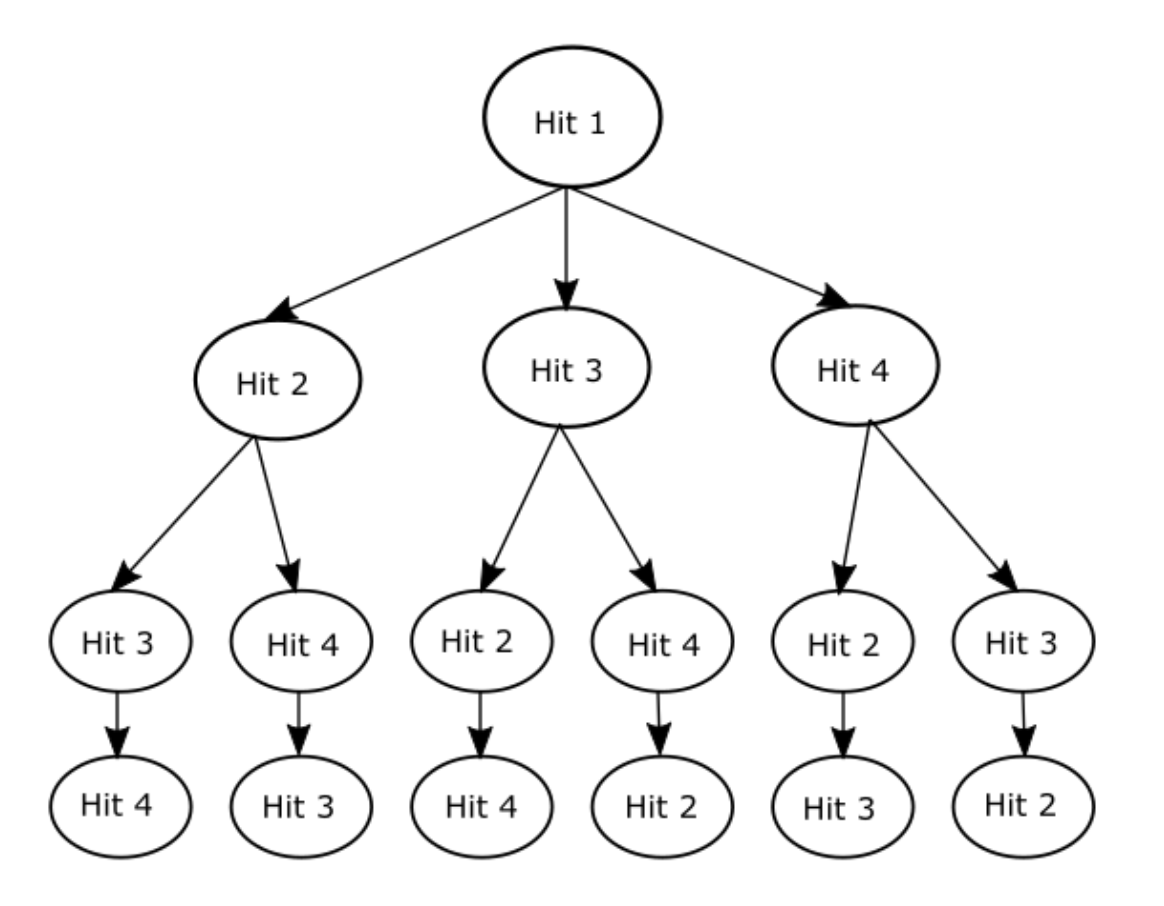
\includegraphics[width=0.6\textwidth]{tree_search_graphic.png}
    \caption{Visual representation of a tree search for one initial hit.}
    \label{fig:tree}
\end{figure}

\subsubsection{Recursive algorithm}
In our program, we keep track of the $\chi^2$ value for each \texttt{Hit} we add to the sequence. As we cannot start calculating the $\chi^2$ value without at least one triple, we first take each possible pair of hits and run them through our recursive search algorithm (line \ref{ln:combo}, Algorithm \ref{alg:recon}), keeping a running tally of the $\chi^2$ value and updating it for each child node we process (line \ref{ln:chi2}, Algorithm \ref{alg:recurse}). Theoretically, we could still have to process every possible sequence before reaching the minimum $\chi^2$ value, but, as will be discussed in the following sections, there are ways to prune the tree in order to decrease the average runtime. The real performance improvement of the tree, however, comes from the recursive approach itself. In our iterative approach, we recalculated $\chi^2$ for each node, including those which had the same parent sequence (giving them the same $\chi^2$ value). In the recursive approach, we cut down on these repeat calculations by carrying the $\chi^2$ value through each sequence and only adding onto it when we process a new node. 

\begin{algorithm}
\caption{Tree search reconstruction algorithm for one photon}\label{alg:recon}
\hspace{\algorithmicindent} \textbf{Input:} \texttt{x} - a 1D array of \texttt{Hit} values for one event, \texttt{n} - the number of hits in the event
\begin{algorithmic}[1]
    \State // Pre-compute spatial angles, $\eta$:
    \For {i,j,k in permutations(n, 3)} \label{ln:precompute} \Comment{Loop over all triples}
        \State // Calculate spatial angle:
        \State $\vec{x}_{i}, \vec{x}_j, \vec{x}_{k} \gets$ $x$[i], $x$[j], $x$[k] \Comment{Consecutive hit positions}
        \State $\hat{r}_i, \hat{r}_j \gets |\vec{x}_j - \vec{x}_i|$, $|\vec{x}_k-\vec{x}_j|$ \Comment{Unit vectors along photon direction}
        \State triples[i][j][k] = $\hat{r}_i\cdot\hat{r}_j$ \Comment{Save spatial angle}
    \EndFor
    \State
    \State min$\chi^2 \gets \infty$
    \State $r \gets$ \texttt{NULL} \Comment{\texttt{Result} value}
    \State
    \For {i,j in permutations(n, 2)} \label{ln:combo} \Comment{Loop over all possible pairs of \texttt{Hit} indices}
        \State $\chi^2 \gets$ \texttt{findOptRecursive}(i, j, $n$, 0) \Comment{Pass first two hits to tree search}
        \State
        \If{$\chi^2 <$ min$\chi^2$} \Comment{Check for most likely permutation}
        \State min$\chi^2 \gets \chi^2$
        \State $\eta'_0 = 1 + \frac{1}{W_0}-\frac{1}{W_1} \pm \delta\eta'_0$ \Comment{New $\eta$ value}
        \State r $\gets x[i]$, $x[j]$, $\eta'_0$ \Comment{Update \texttt{Result} with first two hits and $\eta'_0$}
        \EndIf
    \EndFor
\end{algorithmic}
\hspace{\algorithmicindent} \textbf{Output:} r - \texttt{Result} with predicted $\eta$ and first two hit indices
\end{algorithm}

\begin{algorithm}
\caption{Recursive function in tree search}\label{alg:recurse}
\hspace{\algorithmicindent} \textbf{Input:} \texttt{i}, \texttt{j} - current and next hit indices, respectively, \texttt{n} - number of hits left, $\chi^2$ - current $\chi^2$ value for the sequence
\begin{algorithmic}[1]
\Function{findOptRecursive}{i, j, $n$, $\chi^2$}
    \State // Base case:
    \If{n == 0} \label{ln:hitsUsed}
        \State \Return $\chi^2$
    \EndIf
    \State
    \For{each unused \texttt{Hit}, index k}
        \State // Calculate the new energy angle:
        \State $W \gets W - \frac{1}{m_e c^2}E_2$ \Comment{Calculate change in energy}
        \State $\delta W^2 \gets \delta W^2 - \frac{1}{m_e c^2}\delta E_2^2$
        \State
        \State // Calculate $\eta'$ and $\delta \eta'$ \Comment{See Equation \ref{eq:new_compton}}
        \State $\eta \gets$ triples[i][j][k] \Comment{$\delta\eta$ is constant spatial noise}
        \State
        \State Calculate new $\chi^2$ value from $\eta, \eta', \delta\eta, \delta\eta'$ \Comment{See Equation \ref{eq:chi2}} \label{ln:chi2}
        \State
        \State Prune the sub-tree, if possible \Comment{See Section \ref{pruning}}
        \State
        \State \texttt{findOptRecursive}(j, k, $n-1$, new $\chi^2$) \Comment{Move on to next two hits}
    \EndFor
\EndFunction
\end{algorithmic}
\end{algorithm}

\subsection{Pre-calculation of $\eta$ values}
Another performance improvement comes from pre-calculating the spatial angles for each triple, shown in Algorithm \ref{alg:recon} line \ref{ln:precompute}. In the sequential/iterative algorithm (\ref{alg:seq}), we calculate $\eta$ for each triple in each sequence, but, unlike $\eta'$, the spatial angle does not change our calculations based on the sequence it is in. As it is only based on the hits in its given triple, we can calculate $\eta$ only once for each possible triple before we start the tree search and fetch the values when they are needed. This reduces the computation time at each step in photon reconstruction, which greatly increases our reconstruction speed.

\subsection{Computational cutoffs} \label{pruning}

During our tree search, we can \textit{prune} some sub-trees by filtering out certain sequences before we reach the final recursion depth. Depending on the input ordering of hits, we could still end up having to search the whole tree for the correct path, but generally these methods will improve our runtime on average. We can prune a sub-tree if:
\begin{enumerate}
    \item \textbf{The $\chi^2$ value is already greater than the running minimum.}
    
    Since we always assume the sequence with the minimum $\chi^2$ is best, there is no need to check orderings which have already exceeded our best value.
    
    \item \textbf{The cosine of the energetically reconstructed angle, $\eta'$, is greater than 1 by some amount, the $\eta'$ cutoff.}
    
    Our algorithm might return an $\eta'$-value greater than 1 if we either have the wrong ordering of hits or if there is significant noise in the measurement, so we only prune the tree for values significantly above 1, to be safe.
    
    \item \textbf{The $\chi^2$ value of a sequence exceeds what we would expect for the length of the sequence.}
    
    The p-value is related to the probability that the $\chi^2$ we calculate (based on a Gaussian assumption of noise) will naturally exceed a given $\chi^2$ value with the same degrees of freedom. In other words, it is the probability that a good ordering would have a $\chi^2$ value higher than the expected one. We use a look-up table such as the one shown in Figure \ref{fig:p-val} to find the maximum allowed $\chi^2$ value at each step in our calculation and cut off any sequence which exceeds it. The degrees of freedom we use in the $\chi^2$ table is the number of hits in the sequence so far. For example, if we choose a p-value of 0.01, it means we will not accept any orderings that have less than a 1\% chance of being correct. Using this with Figure \ref{fig:p-val}, this means we will prune the tree for any $\chi^2$ value greater than 6.635 after one hit, greater than 9.210 after two hits, greater than 11.345 after three hits, and so on.
    
    \pagebreak
    
    \item \textbf{We have reached some maximum defined recursion depth, which we refer to as the \textit{reconstructed hits}}
    
    Though this is not shown directly in the pseudocode, it is implemented by changing the base case in Line \ref{ln:hitsUsed} of our program to stop the program after a certain number of hits have been processed. We then assume that the sequence with the minimum $\chi^2$ at the cutoff point has the minimum overall $\chi^2$, though there is some chance that this is not the case (the exact probability depends on the cutoff point). This serves to decrease our computation time, but it also means that we do not take all of our data into account, which we expect will decrease our accuracy.
\end{enumerate}

\begin{figure}
    \centering
    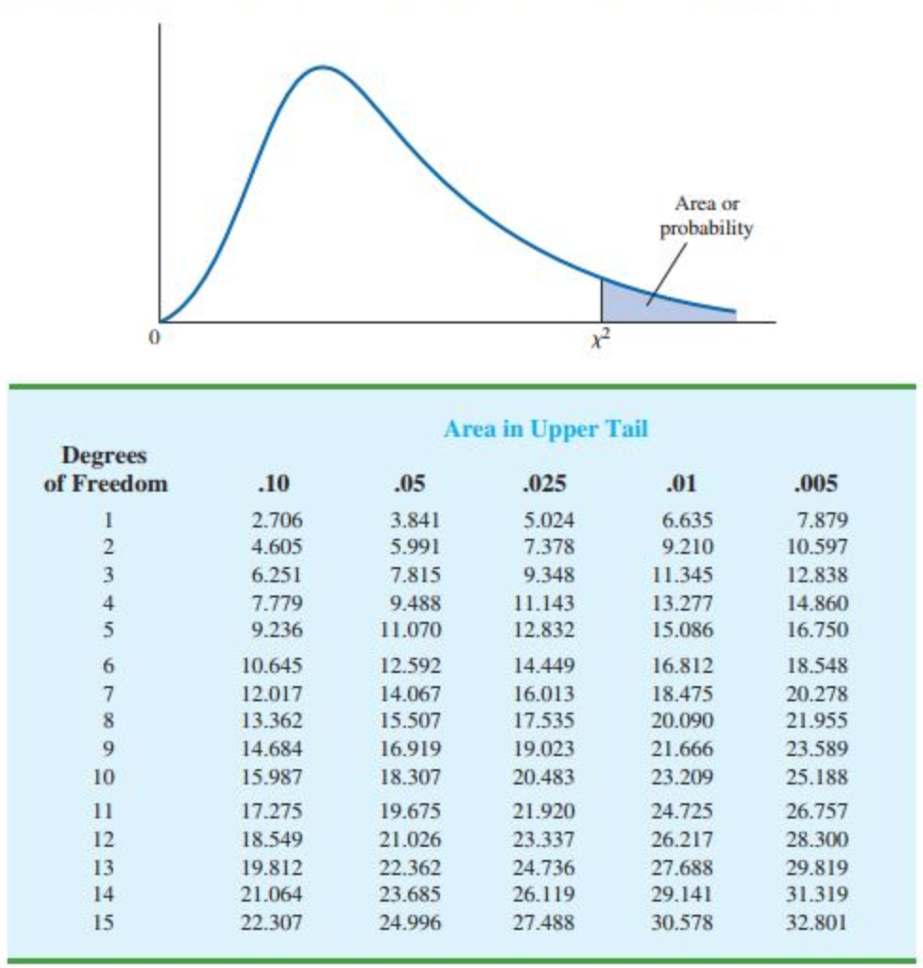
\includegraphics[width=0.5\textwidth]{chi2table.png}
    \caption{An example $\chi^2$ look-up table. \cite{chitable}}
    \label{fig:p-val}
\end{figure}

\section{Parallelism}
Our final performance improvement comes from parallelism. Each photon's computation is independent of the others', so each can be run in a parallel thread to improve the runtime of our algorithm. This also means that if any given photon's computation took longer than expected, there would not be a backlog of events to process which could delay the localization of a gamma-ray burst or other transient. As our current level of parallelism was able to adequately meet our time constraints, we do not seek to increase the reconstruction speed further. However, depending on future time constraints, there are alternate strategies of parallelism and source localization that we could employ to do so.
\chapter{Experiments}

\section{Toy Model Simulator}
Our toy model is a very basic simulator that traces the paths of virtual gamma-ray photons through our detector. This allows us to test code in a controlled environment, which is very useful in the development of our reconstruction algorithm and enables us to ensure our code is performing as we expect without the additional errors caused by outside factors. However, due to this simplicity, there will be physical effects present in the real world that we fail to account for in our simulator, such as background radiation, photon scatters in the detector support material, and various electronic effects, that will increase our overall error. We do not take the detector material into account, nor do we allow for any types of interactions other than a series of Compton scatters followed by a photoabsorption. We set up a test framework on this model simulator that will allow us to adapt our testing to more complicated gamma-ray simulators in the future.

\subsection{Photon simulation} \label{toy_model}
The simulator function, with pseudo-code shown in Algorithm \ref{alg:recon}, takes as its parameters the number of photons to generate and the number of hits each photon should have (including the final absorption). We pick the initial energy of each photon from a uniform distribution between 100 keV and 20 MeV (Line \ref{ln:initE}).

\begin{algorithm}
\caption{Toy Model Simulator}\label{recon}
\hspace{\algorithmicindent} \textbf{Constants:} \texttt{minE}, \texttt{maxE} = 100 keV, 20 MeV - limits on initial photon energy
\hspace{\algorithmicindent} \textbf{Inputs:} \texttt{numEvents} - the number of photons to simulate, \texttt{numHits} - hits per event, \texttt{events} and \texttt{results} - empty arrays for storage
\begin{algorithmic}[1]
\Function{simulate}{numEvents, numHits, events[], results[]}
    \State init alphas[], W[], k[], x[] \Comment{Arrays for the angles, energies, directions,}
    \State \Comment{and hit positions, respectively}
    \For{i in numEvents}
        \State // Initialize variables:
        \State Result \& r $\leftarrow$ results[i] \Comment{Set up result and event references}
        \State Event \& e $\leftarrow$ events[i]
        \State e.hits $\leftarrow$ empty \texttt{Hit} array \Comment{Initialize \texttt{Event} hits}
        \State e.numHits $\leftarrow$ numHits
        \State
        \State // Generate initial energy at random:
        \State r.energy $\leftarrow$ uniform\_random(minE, maxE) \Comment{E $\in$ [minE maxE]} \label{ln:initE}
        \State
        \State // Generate n-1 random angles:
        \State alphas $\leftarrow$ uniform\_random($-\frac{\pi}{2}$, $\frac{\pi}{2}$, n-1) \Comment{Angle array of length n-1} \label{ln:alphas}
        \State r.eta $\leftarrow$ cos(alphas[0]) \Comment{Save initial angle}
        \State 
        \State // Calculate \texttt{Hit} positions, directions, and energies from angles (see \S\ref{toy_model})
        \State calcW(numHits, r.energy, alphas[], W[]) \Comment{Stores energy deposits in W[]} \label{ln:calcW}
        \State calcK(numHits, alphas[], k[]) \Comment{Stores photon directions in k[]} \label{ln:calcK}
        \State calcX(numHits, k[], x[]) \Comment{Stores \texttt{Hit} positions in x[]} \label{ln:calcX}
        \State
        \State perm $\leftarrow$ random permutation of x[] indices \Comment{Randomly shuffle hits} \label{ln:shuffle}
        \State r.p0, r.p1 $\leftarrow$ perm[0], perm[1] \Comment{First two hit indices}
        \State 
        \State // Record each \texttt{Hit}'s position and energy deposit
        \For{j in numHits}
            \State E\_dep $\leftarrow$ (W[j] - W[j+1])*$mc^2$ \Comment{Calculate energy deposit}
            \State e.hits[perm[j]] $\leftarrow$ (x[j], E\_dep) \Comment{Save \texttt{Hit}}
        \EndFor
        \State
        \State addNoise(e) \Comment{Add measurement noise to each hit in the \texttt{Event}} \label{ln:noise}
        \State
    \EndFor
\EndFunction
\end{algorithmic}
\end{algorithm}

Once we have initialized our photon, we simulate its interaction with the detector by generating a random set of scattering angles according to the input number of hits (Line \ref{ln:alphas}). The scattering angles are taken from a uniform distribution from -90 to +90 degrees. We do not simulate back-scatters ($\geq$ 90 degrees), since these are relatively unlikely in the real world. We then use formula \ref{eq:compton} to calculate the energy deposited for each generated scattering angle and store these values in an array (Line \ref{ln:calcW}, \texttt{calcW}).

After calculating the angles and energy deposits, we then must calculate the position of each hit in the detector. To do this, we need to first determine which layers of the detector the photons will scatter in and the vector directions between each pair of hits. This takes place in our function \texttt{calcK} on line \ref{ln:calcK} of our algorithm: for each scatter, we determine the layer of each hit based on an exponential probability distribution, calculate the scattering direction vector by adding the scattering angle (with a random $\phi$ angle) to the photon's previous direction, and save the direction vectors in array \texttt{k}. We can then use simple vector addition to determine the \texttt{Hit} positions and save them in array \texttt{x}, Line \ref{ln:calcX}. We randomly shuffle the hits (Line \ref{ln:shuffle}) in order to simulate the unknown ordering of hits in the detector. If we saved the hits in sequential order for each photon it might cause our program runtime to be shorter than is realistic. Our last step, Line \ref{ln:noise}, is to simulate some random detector noise and add it to each position and energy measurement. The distributions and parameters we use to generate this noise are discussed in the next section.

\subsection{Errors and noise} \label{noise}
We simulate noise in our detector using a Gaussian distribution with variable standard deviation, $\sigma_S$. For the position measurements, the user inputs the standard deviation in millimeters, and for the energy measurements, the standard deviation is input as a constant factor of the energy, $a$:
\begin{equation}\label{eq:sigE}
\frac{\sigma_E}{E} = a*\frac{1}{E \; (keV)}
\end{equation}
We expect based on previous tests of the detector material that $\sigma_S$ will be about 1 mm and $a$ will be about 0.22.

Though the uniform distribution we generate our scattering angles from does not reflect the correct Compton cross-section, our use of Formula \ref{eq:compton} ensures that no interaction we generate would be impossible in nature. As our reconstruction algorithm only compares the inferred angles to the true angles and does not take the scattering cross-section into account either, this simulator still provides a fairly good test of our performance in the absence of systematic measurement error. The true distribution of scattering angles is determined by the Klein-Nishina formula and the interaction probability by the Thomson cross-section \cite{klein-nishina}, so in later iterations of this project it may be useful to incorporate these into our toy model, particularly if we choose to integrate some component of the true scattering probabilities in our reconstruction algorithm.

\section{Hardware}
The hardware we use to test our algorithm is the Raspberry Pi 3, Model B+. It uses a 4-core ARM processor with a 1.4 GHz processing speed, and has 1 GB of RAM. Due to its low number of cores and static execution, it is a slower processor than found in most laptops, but it is perfect for testing our software as it is low-power enough to be used as part of a space telescope. The ARM processor is commonly used for scientific applications, and because NASA has recently commissioned a space processor based on the same architecture, the Raspberry Pi could be the closest hardware available to what our program will actually be running on in space. We tested our parallelism on Cassini, a more advanced machine at Washington University, to get a more accurate measure of our core speedup in Section \ref{parallel}.

\section{Performance Measures}
We use two main performance measures to evaluate our algorithm - the number of photons processed per second, and the accuracy. We consider a reconstruction accurate if the first two hits of the reconstruction match the first two hits in the correct sequence, and refer to this measure as the "two-hit accuracy", or simply the accuracy. We report this statistic as the number of accurate reconstructions over the number of total reconstructions. We also consider power consumption to be a measure of performance, but any trends in power are not studied in-depth as we are well below our expected limit.

\section{Parameters tested} \label{vars}
There are many variables that have the potential to affect the algorithm's performance, and we want to specifically examine the trade-offs in reconstruction speed vs. accuracy for several key parameters. The tests we run are as follows:

\begin{enumerate}
    \item Power - We use the WITRN U2 USB Power Monitor to test the power used by the Raspberry Pi both when it is idle and when it is running our program.
    \item Single vs. double precision - As our program is written in C++, we have a choice of whether to use \texttt{float} values (single precision) or \texttt{double} (double-precision) values in our calculations. Single precision values use fewer bytes than double values, making them faster to use in calculations but sometimes less accurate due to rounding error.
    \item Simulated hits - The number of hits we simulate for each event.
    \item Reconstructed hits - The number of hits we use to reconstruct a photon's trajectory. We cut off computation once the specified number of hits is reached, after which the sequence with the lowest $\chi^2$ value so far is presumed to be the correct one. (i.e. we set a lower-depth base case in Line \ref{ln:hitsUsed} of Algorithm \ref{alg:recurse}).
    \item $\chi^2$ cutoff - The p-value we use for our cutoff $\chi^2$ values. Ex: a p-value of .1 would give us a 10\% probability of cutting off each good triple, whereas a p-value of .01 would give us a 1\% probability of doing so.
    \item $\eta'$-tolerance - The amount above 1 or below -1 that we will allow for a calculated cos(energy angle). For example, if the $\eta'$-tolerance is 0.2, any sequences containing an $\eta' > 1.2$ or $< -1.2$ would be cut.
    \item Predicted spatial and energy noise levels - Our $\chi^2$ calculations rely on the predicted errors of our $\eta$ and $\eta$ values, so changing the predicted level of error will change the behavior of our algorithm. We vary the $\sigma_E$ and $a$ values found in Section \ref{noise} and investigate the results.
    \item Simulated spatial and energy noise - We investigate the interplay between the predicted noise and the simulated noise in both the spatial and energy regimes. Though we have no control over the noise levels we will encounter in operation, it is useful to simulate a range of noise levels and adjust our predicted noise parameters accordingly. This is also useful as a proof-of-concept, as we can check to make sure our algorithm is behaving as expected under increased noise thresholds.
\end{enumerate}
\chapter{Results}
- Each test is run with several basic values that remain unchanged unless otherwise specified: 
- We use 5-hit events, with all 5 hits used in the reconstruction, energy and spatial noise at close to real values (.22 energy noise, 1 mm of spatial noise) and the predicted noise at the same levels
- Each error bar is calculated under the assumption of Gaussian noise, with a p-value of .005
- 

\section{Power}

- We use the WITRN U2 USB Power Monitor to test the power when it's idle and when it's running
- Once plugged in, it displays the average power used and the max power used
- We tested it for a half hour in idle mode - x watts
- We tested it after running our program for 5 minutes - x watts
- We tested it after running for about a half hour - x watts
- This isn't the final hardware, so it probably wouldn't mean much to report the exact values, but the hardware on the APT will be similar, so we expect it to be a good estimate
- draws about 2-4 watts when it's running
- this is well below the 50W we needed to keep under (from Jim), so I think we're good

\section{Precision}
- on a pi, single precision is 32-bit and double precision is 64-bit
- single precision: $3.848x105 \pm 0.513x10^5$ photons/sec vs. double: $5.076x10^5 \pm 0.698x10^5$ photons/sec
- x trials, x photons per trial
- accuracy: 86.12\% vs 86.15\% for accuracy. Not enough that it would make a huge difference for our purposes since our measurements' noise threshold will probably account for a greater error than that.
- since the pi is an in-order processor, it runs comparatively slower with double-precision values than if it were an out-of-order processor
- Using double-precision values reduces rounding error, but it does not give us enough of an increase in accuracy to warrant the reduction in speed.

\section{Parallelism}
- Tested on Cassini because it has more cores
- We run our algorithm on different numbers of cores and calculate the speedup of each trial
- We are using a constant workload for each run, so the speedup in the latency is the sequential execution time divided by the parallel execution time.
- The speedup in throughput is the number of cores used for each run multiplied by the speedup in latency for each run.
- Shows an overall linear trend in speedup, which means that our program has good scalability.

\begin{figure}
    \centering
    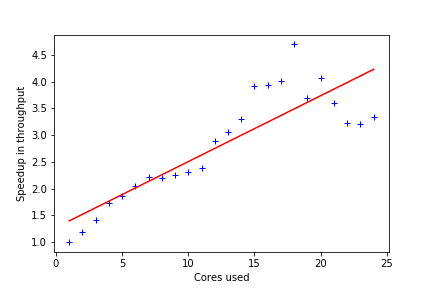
\includegraphics[width=0.7\textwidth]{graphs/Cassini_throughput_speedup.png}
    \caption{Speedup of reconstruction algorithm in throughput.}
    \label{fig:through_speedup}
\end{figure}

\section{Differing numbers of hits}
- Accuracy peaks at about 5 hits, which is interesting
- Speed looks like it goes down exponentially with number of hits, which was also expected (but better than factorial time?)

\section{Hits used in reconstruction}
- Accuracy seems to tail off around 6-8 hits for the toy model
- photons/sec goes down pretty linearly as we increase hits used
- if we get better simulations with Geant we can change the number of hits we use based on the number of hits we receive to maximize our accuracy while minimizing the time spent on each photon

\begin{figure}
    \centering
    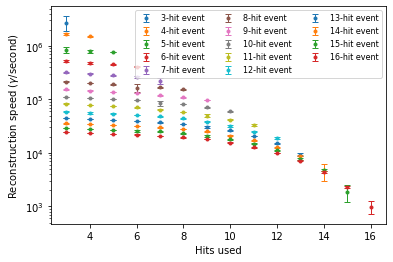
\includegraphics[width=0.7\textwidth]{graphs/pi_hits_v_hitsUsed_speed_final.png}
    \caption{Decrease in throughput with hits used in reconstruction}
    \label{fig:hits_v_hitsUsed}
\end{figure}

\section{p-value}
- visible correlation, but try to get a better one
- speed idk, could increase could decrease, get better error values

\section{$\eta$-tolerance}
- found no real correlation, just noise

\section{Estimated Noise}
- estimated energy noise has a clear downward trend, but over a pretty small range of accuracies
- spatial noise not so much, perhaps increase the range

\section{Simulated Noise}
- helps with proof of concept
- we expect accuracy to go down with increased noise, and it does for both
\chapter{Conclusion}

\section{Discussion}
As part of this project, we developed and tested a model simulator for gamma-ray trajectories, wrote a Compton reconstruction algorithm, and set up a framework for testing and investigating trends in our data. We have met our constraints for power and better constrained our accuracy and reconstruction speeds based on possible input parameters and simulated environmental factors.

Our overall goal was to be able to reconstruct at least 50,000 photons per second with greater than 75\% accuracy, and, based on our findings in sections \ref{totalhits} and \ref{reconhits}, we will be able to achieve this goal by implementing a maximum cutoff in the number of reconstructed hits for each event. Based on our data in Figure \ref{fig:hits_speed}, we have also been able to improve the average-case time complexity of our program from factorial to exponential with our tree search algorithm. Our program has, on average, a linear trend in speedup, indicating that it scales well, though we will likely have a maximum of four cores to work with if the telescope uses a standard ARM processor in its hardware.

Though we saw mostly expected behavior when testing the various parameters, there are a few interesting features which may prove useful to future work on this project. In varying the number of hits for each event, we found an unexpected trend in accuracy that may help us better reconstruct the position of a gamma-ray source in future iterations of the project. While investigating reconstructed hits, we found that stopping computation early could save us computation time without significant loss of accuracy. Finally, in varying our predicted noise levels, we found that the point at which the accuracy flattens out is a fairly good predictor of the simulated energy noise in our system. This could help us better determine the true noise level when performing tests with real telescope equipment.

\section{Future Work}
Though this project laid the groundwork for the simulation and reconstruction of Compton scatters for our detector, there is much left to do before the telescope becomes fully operational. One of the primary goals of future projects will be to repeat the test cases we have performed on more accurate data from CERN's Geant 4 simulator to make sure that we see the same behavior from both. An alternative approach could be to make our toy model simulator more robust by simulating events from a given gamma-ray source profile and by including the correct probability distributions for Compton scattering angles. Once this is finished, the next logical step would be to include the Klein-Nishina formula as a prior on our reconstruction algorithm, which would prioritize triples of hits more likely to be Compton scatters based on the angle itself, rather than just comparing the energy and spatial angles to see if they match. Compton scatters are much more likely to happen at small angles for our energy range, so including this in our calculations could further improve our reconstruction accuracy.

Testing on a better simulator would also allow us to examine the overall accuracy of our program for different source distributions rather than just the accuracy for events with a given number of hits. In our current tests, all events have equal weight, whereas Compton scatters in nature are much more likely to have 2-3 hits than any larger number. This means that the overall accuracy would be a weighted mean of those we found in section \ref{totalhits}, with the overall shape of the distribution depending on the emission distribution of the source. With these probabilities taken into account, we would potentially be able to optimize our program for the expected source distribution. Correct figures for the accuracy would also be very useful as a prior on the source reconstruction algorithm, which has yet to be developed.

The use of parallelism in our algorithm also requires some further investigation. The current program runs each photon in parallel, but theoretically each branch of our tree search could also be done simultaneously. There would be a small amount of overhead associated with the creation of each parallel thread, so at some point the extra parallelism would cease to be worth the decreased speed. Though we are meeting our speed goals currently, it would be interesting to investigate the optimal level of parallelism for a program such as this, in case it is needed in the future. 

- we need to get the geant data to work
- we need to investigate these trends further in the Geant data
    - events with more hits are less likely, so that will affect our accuracy
    - in our current graphs we are giving all events equal weight, which is not a good approximation of real Compton scattering
    - we should do a cost/benefit analysis with that taken into account, and perhaps we would be able to cut even more hits than these graphs suggest
    - we would expect to see something like the sum of our graphs weighted by the probability of each number of hits
- make toy model simulator better (real probabilities for interaction, etc)
- investigate whether further parallelism would be of use (in the loop) or if it would simply bog down the computation with more overhead time.

- Though we use $\chi^2$-pruning on our tree search algorithm, we still are performing this operation sequentially within each of our parallel threads. We have not implemented this parallelism yet since we have already reached our current timing goals, but if we ever need to improve the runtime further we could always introduce parallelism into the tree search itself. (*** future work section) The height of the tree is only N nodes, where N is the number of hits, so theoretically we could reach a linear time for that part of our algorithm, though in practice we would need N! processors to acheive this kind of speed improvement, not to mention the overhead time that the creation of each parallel thread would need. It is not clear what kind of speed improvements we would see in practice, but it may be useful to investigate this in future projects.

- through a tree search, we were able to improve the average-case runtime of our program from factorial time to exponential time, and reach our throughput goals with the use of parallelism and code optimization.\\
- our parallelism gives us an (on average) linear trend in speedup, though, as there are only 4 cores on a standard ARM processor, we don't expect an extreme speed boost from this fact.\\
- we set up a framework for plotting relevant quantities which can be used to test future simulations for this project\\
- we saw somewhat expected results for hits data and energy/spatial noise\\
- have not found a peak in the p-value plot, so the best plan seems to just be to use the lowest value we've tested.\\
- biggest things to focus on are the hits to hits used and the trend in estimated energy noise\\
- by limiting our reconstruction of certain events, we can increase our throughput while maintaining a similar overall accuracy (reference numbers)\\
    - since higher numbers of hits are less common, the deficit in accuracy is almost guaranteed to be smaller than the one predicted in this paper for each cutoff of \#hits\\
- The trend of predicted energy accuracy shows that our accuracy increases as we get closer to the true value (for a given number of hits)\\
    - if this holds with the Geant data, it is a good way to get an estimate of the true energy noise, and we can then set that value to give us the best accuracy we can.\\

%\appendix                        % now we start appendicies
%\chapter{Pseudocode}
\label{app:code}

%%% Sequential & iterative algorithm
\begin{algorithm}
\caption{Sequential Reconstruction Algorithm Part 1}\label{recon1}
\begin{algorithmic}
\For {each photon}
    \State $n \gets$ \# hits for photon $i$
    \State min$\chi^2 \gets$ max double
    \State bestPermutation $\gets 0$
    \For {permutation $j \in$ all $n!$ permutations}
        \State $\chi^2 \gets 0$
        \For {hit $k\in 1...n-1$}
            \State // Calculate spatial angle:
            \State $\vec{x}_k \gets$ position of hit k
            \State $\hat{r}_k \gets |\vec{x}_{k+1} - \vec{x}_k|$ \Comment{Unit vector along photon direction}
            \State $\eta_k = \cos{\phi_k} = \hat{r}_k\cdot\hat{r}_{k-1}$ \Comment{From dot product equation}
            \State
            \State // Calculate energy angle:
            \State $W_k = \frac{1}{m_e c^2}\sum_{i=k+1}^n E_i$ \Comment{Unitless energy; energy before hit k}
            \State $\eta'_k = \cos{\phi'_k} = 1 + \frac{1}{W_{k-1}}-\frac{1}{W_k}$ \Comment{From Compton equation}
            \State
            \State // Calculate Errors:
            \State $\delta\eta_k^2 = \delta\phi_{k,r}^2\sin^2(\phi_k)$ \Comment{$\delta\phi_{k,r}$ depends on $\delta x,\delta y,\delta z$}
            \State $\delta\eta'^2_k = \frac{\delta W_{k-1}^2}{W_{k-1}^4}+\delta W_k^2 \big[(\frac{1}{W_k^2}-\frac{1}{W_{k-1}^2})^2 - \frac{1}{W_{k-1}^4}\big]$
            \State
            \State // Add to $\chi^2$:
            \State $\chi^2 \gets \chi^2 + \frac{1}{n-2} \frac{(\eta_k-\eta'_k)^2}{\delta\eta_k^2 + \delta\eta'^2_k}$
        \EndFor
        \algstore{break}
\end{algorithmic}
\end{algorithm}
    
\begin{algorithm}
\caption{Sequential Reconstruction Algorithm Part 2}\label{recon2}
\begin{algorithmic}
        \algrestore{break}
        \State
        \If{$\chi^2 <$ min$\chi^2$}
        \State min$\chi^2 \gets \chi^2$
        \State bestPermutation $\gets j$
        \EndIf
    \EndFor
    \State
    \State // Predict $\eta$:
    \State $\eta_{pred} = 1 + \frac{1}{W_0}-\frac{1}{W_1} \pm \delta\eta'_1$
    \State
\EndFor
\end{algorithmic}
\end{algorithm}

\iffalse

While this guide answers most questions about how to format a thesis, it does
not address questions about English grammar, use of abbreviations, punctuation,
spelling, and other confusing subjects.  Students should obtain a dictionary
and a style of grammar book to refer to as questions arise.  The dictionary is
important because most electronic spelling checkers are not complete and do not
contain definitions.  (You may also need to refer to some of the references you
cite for the spelling of technical terms.)  The grammar or style book is useful
for checking grammar and punctuation rules.  A good style manual contains
information about correct English usage as well as advice for preparing a
manuscript.  \textit{A Manual for Writers of Term Paper, Theses, and
Dissertations}~\cite{Turabian} is one such concise and inexpensive manual based
on the lengthy and more expensive \textit{Chicago Manual of
Style}~\cite{ChicagoManual}.  

The following rules will help you avoid three mistakes frequently made
by students:
\begin{itemize} 
 \item Hyphenated words must begin and end on the same page.

 \item When a page break falls in the middle of a paragraph, at least
two lines of text from that paragraph must appear on the second page.

 \item At least one line of text from a section or subsection must
appear on the same page as the title of that section or subsection.
\end{itemize}

%%% Local Variables: 
%%% mode: latex
%%% TeX-master: "thesis-main"
%%% End: 
\fi
%\chapter{Procedures and Deadlines}
\label{app:procedures}

\paragraph{Deadlines}

At least one semester prior to the semester in which you believe you will
complete all requirements for your degree, please be sure to consult with your
department's graduate administrative assistant or coordinator to be sure you
are aware of all requirements and deadlines with regards to the submission of
your thesis or dissertation.  Deadlines are printed in the course listings
schedule book and are posted online.  If you cannot make certain deadlines, you
may have to postpone your graduation accordingly.  In particular, a student
must file an ``intent to graduate'' form (via WebSTAC) by the published
deadline prior to any anticipated graduation date; otherwise, no degree can be
earned.  M.S.\ and D.Sc.\ students also have a special deadline by which they
must submit an initial draft (PDF) of their thesis to Engineering Student Services 
at \uline{ess@seas.wustl.edu}  to be reviewed for formatting.  After a
draft has been submitted for format review, an email will be sent to you within
48 hours detailing any changes that need to be made in the formatting of your
thesis or dissertation.  For M.S.\ and D.Sc.\ students, approval of your thesis
or dissertation formatting must be received prior to turning in the final
electronic and hard copy versions as described below.  

Ph.D.\ students must follow the requirements of the Office of Graduate Students
in Arts and Sciences (GSAS).  The GSAS office does not have special formatting
deadlines, but you should still contact that office if you have questions about
your formatting.

\paragraph{Oral Examination}

Each member of the oral examining committee must be given a copy of the thesis
or dissertation, in final form, in sufficient time to study it before the oral
examination.  Members of the examining committee have the right to request
rescheduling of the examination if these copies are not made available to them
at least one week in advance of the scheduled examination date.  Copier paper
may be used for these preliminary copies.

\paragraph{Electronic Submission}

After the oral defense, an M.S.\ or D.Sc.\ student is required to submit an
electronic version of his/her final thesis or dissertation in PDF format.  The
links can be found on the Engineering Student Services website under the Graduate
Student Services section.  Click on the link for Thesis and Dissertation Submissions 
and then select the appropriate link for Master's or D.Sc. electronic submission under 
step 3. The website for doctoral students submitting
dissertations requires students to choose among publishing and copyrighting
services offered, but the University permits students to make whichever choices
they prefer. Doctoral students are asked to submit a Survey of Earned
Doctorates separately to Engineering Student Services. 

Please note that the electronic submission of your thesis or dissertation
should be made by the stated deadline date on the current academic calendar and
prior to handing in the final hard copies as described below.  An administrator
in Engineering Student Services will review the electronic copy of your thesis
or dissertation and officially approve the submission online.  This electronic
version will be used for library publication and catalog purposes. In addition,
students typically must submit hard copies of the thesis or dissertation for
binding purposes (see below).  

\paragraph{Final Hard Copies}

After the oral defense and electronic submission, final copies of the thesis or
dissertation approved by the examination committee and department are to be
submitted to Engineering Student Services in Lopata 303 on or before the date
stated in the current academic calendar.

\begin{enumerate}
	\item	
	\textbf{Three} final copies (unless your department instructs you
	otherwise) must be printed using only one side on 8.5 $\times$ 11 inch
	white paper and minimum 20-pound weight. (Most printer and copier paper
	qualify, but a high-quality watermarked or 10--25\% cotton paper is
	recommended.) Print should be letter quality.  Copies submitted should
	\uline{not} be bound, stapled, clipped or hole-punched.  To avoid
	delays in publication, please make certain that the copies you submit
	include all pages of your thesis or dissertation.
	
	Each copy should be placed in a separate unsealed manila envelope with
	a copy of the \textbf{short title page} (see description below)
	securely taped to the outside of each envelope.

	\begin{list}{}{}
		\item \textit{%
		Engineering Student Services sends all three copies of your
		thesis or dissertation to West Campus Library.  The Library
		will have these copies professionally bound and sent back to
		your home department.  The home department will keep one copy
		and distribute one to your advisor.  The third copy will be
		mailed to you at your home address.  In order for you to
		receive your bound thesis or dissertation promptly, your home
		department must have your current mailing address.  On your
		``intent to graduate'' form you should input your ``address
		after graduation.''   Processing theses and dissertations takes
		time, so you may have to wait 3--6 months after your graduation
		date to receive your copy. 
		}
	\end{list}

	\item		
	\uline{\textbf{Short Title} page is a loose sheet containing} (1) a
	\uline{short title} of 35 letters or less (including spaces), (2) the
	author’s last name, (3) the degree, and (4) the year of its award,
	centered on the page and punctuated as in the example.\footnote{See the
	sample short title page at the end of this document}    This short title sheet is
	to be taped securely to the outside of each manila envelope as
	described above.  This information lets the bindery know what to put on
	the spine of the bound copies.  The title will be truncated if longer
	than 35 characters.
	
	\item
	\textbf{Doctoral (D.Sc.) degree candidates} must complete the Survey of
	Earned Doctorates form and submit it with the 3 copies of your final
	dissertation. You can download the Survey of Earned Doctorates form
	from the School of Engineering's website under Graduate Student
	Information and Forms.

	\textbf{NOTE FOR PH.D.\ STUDENTS}:  Deliver all three copies of your
	dissertation to the GSAS Office.  See GSAS dissertation guidelines on
	their web site.
\end{enumerate}

%%% Local Variables: 
%%% mode: latex
%%% TeX-master: "thesis-main"
%%% End: 

%\chapter{Thesis Format Checklist}

\newcommand{\smallblank}{\underline{\hspace{0.25in}}\,}
\newcommand{\largeblank}{\underline{\hspace{0.75in}}\,}

{\footnotesize \textbf{NOTE: If you have significantly varied formatting from that
which is shown in this document, please complete this form and submit it to
Engineering Student Servcies when you submit your thesis for format review.}}

Author's Name:  \underline{\hspace{4.0in}} \\
Title page font:  \smallblank 12 pt \indent \smallblank 14 pt \\
Table of contents chapter titled font: \smallblank plain \indent \smallblank bold \\
First level table of contents indentation (0 to 0.5 inch): \largeblank \\  
Second level table of contents indentation (0 to 1 inch): \largeblank \\
Body text font: \smallblank 10 point \quad \smallblank 11 point \quad \smallblank 12 point \\
Body text line spacing: \smallblank 1.5 \quad \smallblank 2 \indent \\
Body text justification: \smallblank left \quad \smallblank full \\
Paragraph indentation (0 to 0.5 inch):  \largeblank \\
Chapter title position (1.5 to 3 inches below top edge):  \largeblank \\
\begin{tabular}{@{}lll}
Chapter title style: \smallblank with word ``Chapter'' & \multicolumn{2}{l}{\smallblank without word ``Chapter''} \\
Chapter title:  \smallblank (10 to 36 point) & \smallblank plain & \smallblank bold \\
& \smallblank centered & \smallblank left justified \\
Section heading: \smallblank (10 to 24 point) & \smallblank plain & \smallblank bold \\
& \smallblank centered & \smallblank left justified \\
Subsection heading:  \smallblank (10 to 18 point) & \smallblank plain & \smallblank bold \\
& \smallblank centered & \smallblank left justified \\
Unnumbered heading: \smallblank (10 to 14 point) & \smallblank plain & \smallblank bold \\
& \smallblank centered & \smallblank left justified
\end{tabular} \\
Label tables as: \smallblank Table \quad \smallblank Figure \\
Reference list style (parenthetical, etc.): \underline{\hspace{3.0in}}

%%% Local Variables: 
%%% mode: plain-tex
%%% TeX-master: t
%%% End: 

%\wrappedappendix{Special Notes for \LaTeX{} Users, Including a \\
	\hbox to 1.0in{}Demonstration of Wrapping Appendix Titles}
{Special Notes for \LaTeX{} Users, Including a Demonstration of Wrapping Appendix Titles}
%\chapter{Special Notes for \LaTeX{} Users}
\label{app:latex-notes}

\newcommand{\cmd}[1]{\texttt{$\backslash$#1}}

It is strongly recommended that you use this file as a template for your
thesis, since it greatly simplifies conforming to the required formatting
standards.

There are several important points that students using the \LaTeX{} version of
this template should verify before submitting a thesis.

\section{Front Matter}

Much of the front matter (i.e., the Roman numbered pages) is automatically
generated.  Use \cmd{renewcommand} command to customize the fields of these
templates.  For example,
\texttt{\cmd{renewcommand}$\{$\cmd{thesisauthor}$\}\{$your name here$\}$} will
customize the author name.

\sloppy
Most authors will need to customize the \cmd{thesismonth}, \cmd{thesisyear},
\cmd{thesisauthor}, \cmd{thesisauthorlastname}, \cmd{thesisdefensedate},
\cmd{thesistitle}, \cmd{thesisshorttitle}, \cmd{thesisdepartment},
\cmd{thesisfield}, \cmd{thesissupervisor}, and \cmd{thesiscommittee}
fields.  Examples of these can be seen in the sample \texttt{thesis-main.tex}
file.

\fussy
You must also specify \texttt{phdthesis}, \texttt{dscthesis}, or
\texttt{mastersthesis} when selecting the \cmd{documentclass}.  An
example can also be seen in the sample \texttt{thesis-main.tex} file.

\section{Table of Contents and Bibliography}

The Table of Contents is automatically generated.  \texttt{latex} should be run
twice in succession after making any changes to the Table of Contents.

Due to the way \LaTeX{} formats the Table of Contents, long appendix titles
will not automatically wrap and indent properly.  If you need to use a long
appendix title, you must manually wrap and indent the appendix's
table-of-contents entry.  The \cmd{wrappedappendix} command is defined in this
template to assist with this; an example is seen at the top of the sample
\texttt{thesis-appendixD.tex}.  This requirement only applies to appendix
titles: other section titles will automatically wrap properly, including
entries in the List of Tables and List of Figures.

If changes need to be made to the Table of Contents' formatting, you can use
the \cmd{addtocontents} command to insert some formatting commands
directly into the Table of Contents page.  More significant changes can be made
by editing the \texttt{.toc} file that \LaTeX{} automatically generates.
However, editing this file by hand is not recommended unless absolutely
necessary, since it will automatically be re-generated the next time \LaTeX{}
is run.

Like the Table of Contents, the Bibliography is automatically generated.  After
editing the bibliography file, you should run \texttt{latex}; run
\texttt{bibtex}; and re-run \texttt{latex} twice in succession.

\section{Widows and Page Breaks}

\LaTeX{} may create widows if you have a paragraph followed by a list.  To get
rid of this widow, you must force \LaTeX{} to break the page somewhere else.
Either insert a \cmd{newpage} command before the paragraph, or insert a
\cmd{samepage} command between the paragraph and the list.

\LaTeX{} may also create widows in the Tables of Contents.  You can force
\LaTeX{} to break the page in a more convenient location by inserting
\cmd{addtocontents$\{$toc$\}\{$\cmd{newpage}$\}$} before the corresponding
\cmd{chapter}, \cmd{section}, \cmd{subsection}, or \cmd{subsubsection} command
in the text.

Excluding these two situations, \LaTeX{} should not create orphans or widows.
However, in some situations it may place page breaks at strange places --- such
as several inches above the bottom margin --- in order to avoid creating
orphans or widows.  You can fix this by altering the \cmd{clubpenalty} or
\cmd{widowpenalty}, or by manually adding \cmd{newpage}s where \LaTeX{} guesses
incorrectly.


% A good place for the bibliography.
%
\bibliographystyle{plain}
\begin{spacing}{1.0}
\bibliography{./thesis-references}
\end{spacing}
\nocite{*}
%
% The Vita should be the last thing
%
\begin{thesisauthorvita}
%
% This is just a sample of what to do in a vita
%
%
%
% Sample  Vita
% This is done in a list environment.
%
% Personal heading
\begin{center}
{\large\thesisauthor}
\end{center}
%
% Need to 'fold' long labels
%
\newcommand{\vitalabel}[1]%
  {\raisebox{0pt}[1ex][0pt]
    {\makebox[\labelwidth][l]%
      {\parbox[t]{\labelwidth}{\hspace{0pt}\textbf{#1}}}}}
%
% Here's the list definition
%
\begin{list}
  {}%                                        nodefault label
  { \renewcommand{\makelabel}{\vitalabel}%   setting labels
    \setlength{\labelwidth}{100pt}%          label width
    \setlength{\leftmargin}{120pt}%
    \setlength{\itemindent}{0pt}%            don't indent first line of items
    \setlength{\parsep}{\baselineskip}%               space between paragraphs
    \setlength{\itemsep}{5pt}%               additional space between items
    }

\item[Degrees] B.A.\ Magna Cum Laude, Physics, August 2018 \\
\item[Professional\linebreak Societies]
  Phi Beta Kappa Honor Society \\
  Sigma Pi Sigma Honor Society\\
  \iffalse
\item[Publications]
  Student, I.\ D.\ (2005).\ \LaTeX{} document class for Sever Institute,
  \textit{The \LaTeX{} J.} \textbf{10}(4):~323--336.
  
  Student, I.\ D.\ (2005).\ More \LaTeX{} wisdom, \textit{Another \LaTeX{} J}.
  \textbf{42}(7):~100--101.
  \fi
\end{list}
\flushright
\thesismonth\ \thesisyear


\end{thesisauthorvita}
\iffalse
{\flushleft
\textit{Note:} Use month and year in which your degree will be conferred.}
\fi

\begin{thesisshorttitlepage}
\iffalse
{\small 

\textbf{NOTE:}	This is a sample of a ``short title'' page.  Please change the
line above to use an appropriate ``short title'' for your thesis, insert your
last name, and include your degree and year in which the degree will be earned.
Separate elements using commas, as illustrated in the sample above.
\uline{Your ``short title'' cannot exceed 35 characters, counting spaces}.  It
does not matter if there is a page number at the bottom of the page.  

\textbf{IMPORTANT:} This page should be printed and taped securely to each of
the three manila envelopes used to submit your final hard copies.  Remove this
page before submitting your final copies (i.e., this page should not be
included in either your electronic submission or your hard copy submissions).
See Appendix~\ref{app:procedures} for further details if necessary.
}
\fi
\end{thesisshorttitlepage}

%%% Local Variables: 
%%% mode: latex
%%% TeX-master: "thesis-main"
%%% End: 


\end{document}
